% Sequence diagram: asking a question (Figure 4.9)
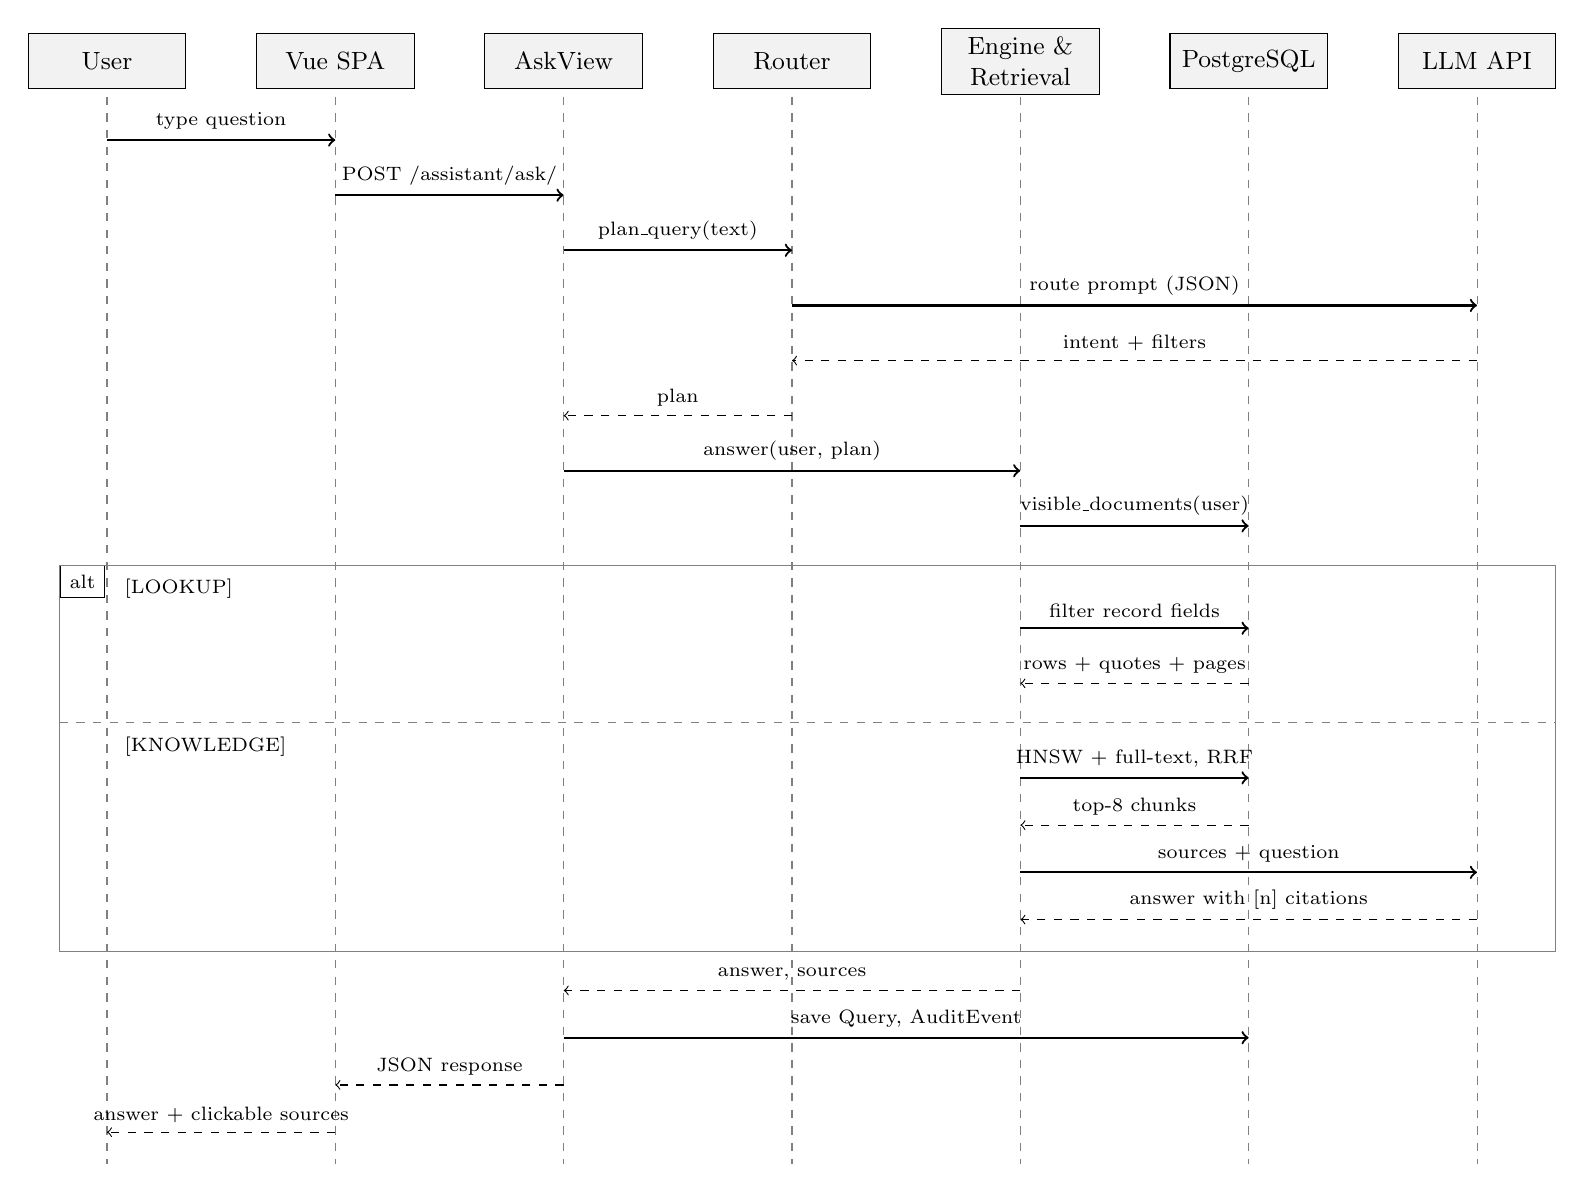
\begin{tikzpicture}[
  ll/.style={draw,fill=gray!10,font=\small,minimum width=20mm,minimum height=7mm,align=center},
  msg/.style={->,thick},
  ret/.style={->,dashed}]
\foreach \x/\n/\t in {0/u/User, 2.9/s/Vue SPA, 5.8/a/AskView, 8.7/r/Router, 11.6/e/Engine \&\\Retrieval, 14.5/d/PostgreSQL, 17.4/l/LLM API}
  {\node[ll] (\n) at (\x,0) {\t}; \draw[dashed,gray] (\x,-0.45) -- (\x,-14.0);}
\def\smsg#1#2#3#4{\draw[msg] (#1,#3) -- node[above,font=\scriptsize]{#4} (#2,#3);}
\def\sret#1#2#3#4{\draw[ret] (#1,#3) -- node[above,font=\scriptsize]{#4} (#2,#3);}
\smsg{0}{2.9}{-1.0}{type question}
\smsg{2.9}{5.8}{-1.7}{POST /assistant/ask/}
\smsg{5.8}{8.7}{-2.4}{plan\_query(text)}
\smsg{8.7}{17.4}{-3.1}{route prompt (JSON)}
\sret{17.4}{8.7}{-3.8}{intent + filters}
\sret{8.7}{5.8}{-4.5}{plan}
\smsg{5.8}{11.6}{-5.2}{answer(user, plan)}
\smsg{11.6}{14.5}{-5.9}{visible\_documents(user)}
\node[draw,font=\scriptsize,anchor=north west,fill=white] at (-0.6,-6.4) {alt};
\draw[gray] (-0.6,-6.4) rectangle (18.4,-11.3);
\draw[gray,dashed] (-0.6,-8.4) -- (18.4,-8.4);
\node[font=\scriptsize,anchor=west] at (0.1,-6.7) {[LOOKUP]};
\smsg{11.6}{14.5}{-7.2}{filter record fields}
\sret{14.5}{11.6}{-7.9}{rows + quotes + pages}
\node[font=\scriptsize,anchor=west] at (0.1,-8.7) {[KNOWLEDGE]};
\smsg{11.6}{14.5}{-9.1}{HNSW + full-text, RRF}
\sret{14.5}{11.6}{-9.7}{top-8 chunks}
\smsg{11.6}{17.4}{-10.3}{sources + question}
\sret{17.4}{11.6}{-10.9}{answer with [n] citations}
\sret{11.6}{5.8}{-11.8}{answer, sources}
\smsg{5.8}{14.5}{-12.4}{save Query, AuditEvent}
\sret{5.8}{2.9}{-13.0}{JSON response}
\sret{2.9}{0}{-13.6}{answer + clickable sources}
\end{tikzpicture}
